\message{ !name(googleVis.Rnw.tex)}
\message{ !name(googleVis.Rnw) !offset(25) }


\author{Markus Gesmann\footnote{markus.gesmann@gmail.com},
  Diego de Castillo\footnote{decastillo@gmail.com}\\
Contact: rvisualisation@gmail.com}
\title{Using the Google Visualisation API with R:\\
  googleVis-\Sexpr{packageDescription("googleVis")$Version} Package Vignette}
\maketitle
\begin{abstract}
  The \googleVis package provides an interface between R and the
  Google Visualisation API.  The Google Visualisation API offers
  interactive charts which can be embedded into web pages. The most
  well known of those charts is probably the Motion Chart, popularised
  by Hans Rosling in his TED talks.  With the \googleVis package users
  can create web pages with  interactive charts based on R data frames
  easily and display them either via the \rsp package or
  within their own sites. Currently the package provides interfaces to
  Motion Charts, Maps, Geo Maps, Tables and Tree Maps. 
\end{abstract}

\clearpage
\tableofcontents
\clearpage

\section{Introduction}

\subsection{Motivation}
More and more data is becoming available and accesible, and yet
stories and insights are still often missed: we are lost in the data
jungle and struggle to see the wood for the trees. 

Hence new tools are required to bring data to life, to engage with
users, to enable them to slice and dice the data, to view it from
various angles and to find stories worth telling: outliers, trends or
even the bleeding obvious.

In 2006 Hans Rosling gave an inspiring talk at TED
~\cite{HansRoslingTedTalk} about social and economic developments in
the world over the last 50 years, which challenged the views and
perceptions of many listeners. Rosling had used extensive data analysis
to come to his conclusions.  To visualise his talk, he and his team at
Gapminder~\cite{Gapminder} had developed animated bubble charts, aka
motion charts, see Figure~\ref{MotionChartGUI}. 

Rosling's presentation popularised the idea and use of interactive
charts, and as a result the software behind
Gapminder was bought by Google and integrated as motion charts into
their Visualisation API~\cite{GoogleVisApi} a few years later. 

In  2010 Sebasti\'{a}n P\'{e}rez Saaibi~\cite{Saaibi2010} presented at
the R/Rmetrics Workshop on  Computational Finance and Financial
Engineering the idea to link motion charts with R  using the
\rsp package~\cite{Rsp}. 

Inspired by those talks and the desire to use interactive data
visualisation tools to foster the dialog between data analysts and
others the authors of this vignette started the development of the
\googleVis package~\cite{googleVis}.

\begin{figure}[!ht]
\begin{center}
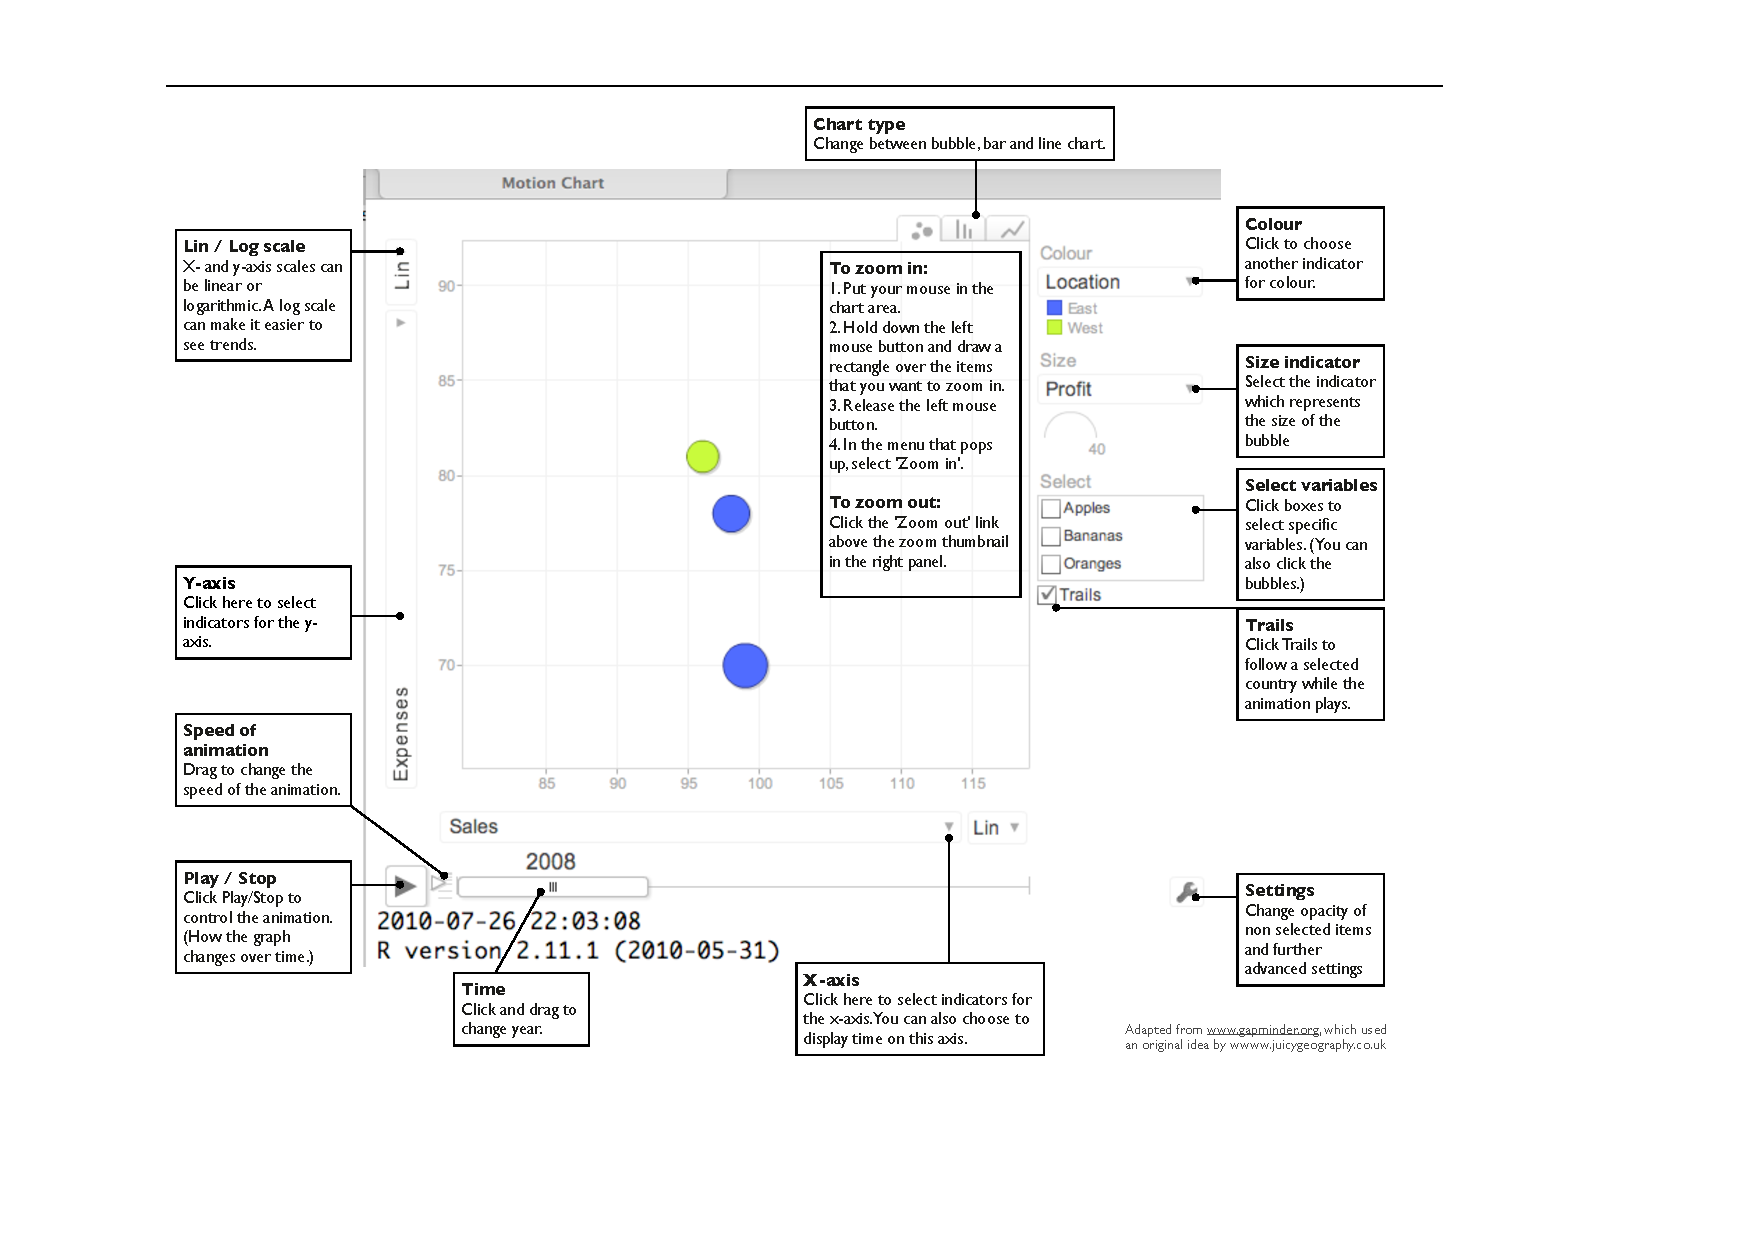
\includegraphics[width=\textwidth]{MotionChart.pdf}
\caption{
  Overview of a Google Motion Chart.  Screenshot of the output of
  \texttt{plot(gvisMotionChart(Fruits, idvar='Fruit', timevar='Year'))}
}\label{MotionChartGUI}
\end{center}
\end{figure}
\clearpage

\subsection{Google Visualisation API}

The Google Visualisation API~\cite{GoogleVisApi}, \cite{GoogleTerms}
allows users to create interactive charts as part of Google
documents/spreadsheets and web pages. In this text we will focus 
on the usage of the API as part of web sites.

The Google Public Data Explorer~\cite{GooglePublicData} provides a
good example, demonstrating the use of motion charts and how they can
help to analyse data. Please note, that all those charts are rendered
within a browser using Adobe Flash~\cite{Flash}.

The charting data can either be embedded into the html file or read
dynamically. Key to the Google Visualisation API is that the data is
structured in a DataTable~\cite{DataTable}, and this is where the \googleVis
package helps, as it uses the functionality of the \rjsonio
package~\cite{RJSONIO} to transform R data frames into
JSON~\cite{json} objects as the basis for a DataTable.

As an example we shall look at the html-code of a motion chart from Google's visualisation 
gallery~\cite{GoogleMotionChart}, which generates output similar to
Figure~\ref{MotionChartGUI}:

\begin{verbatim}
<html>
  <head>
    <script type="text/javascript" src="http://www.google.com/jsapi">
    </script>
    <script type="text/javascript">
      google.load('visualization', '1', {'packages':['motionchart']});
      google.setOnLoadCallback(drawChart);
      function drawChart() {
        var data = new google.visualization.DataTable();
        data.addColumn('string', 'Fruit');
        data.addColumn('date', 'Date');
        data.addColumn('number', 'Sales');
        data.addColumn('number', 'Expenses');
        data.addColumn('string', 'Location');
        data.addRows([
          ['Apples',new Date (1988,0,1),1000,300,'East'],
          ['Oranges',new Date (1988,0,1),1150,200,'West'],
          ['Bananas',new Date (1988,0,1),300,250,'West'],
          ['Apples',new Date (1989,6,1),1200,400,'East'],
          ['Oranges',new Date (1989,6,1),750,150,'West'],
          ['Bananas',new Date (1989,6,1),788,617,'West']
          ]);
        var chart = new google.visualization.MotionChart(
                     document.getElementById('chart_div'));
        chart.draw(data, {width: 600, height:300});
      }
    </script>
  </head>

  <body>
    <div id="chart_div" style="width: 600px; height: 300px;"></div>
  </body>
</html>
\end{verbatim}
You will notice that the above html-code has three generic parts:
\begin{itemize}
\item reference to a javascript function provided by Google, here 
	\texttt{'motionchart'},

\item data to visualise as a \texttt{DataTable}, 

\item chart with chart id (\texttt{'chart\_div'}) and options, here width
  and height. 
\end{itemize}

Those principals hold true for most of the interactive charts of the
Google Visualisation API, see the examples in Figure~\ref{demos}.

To display the visualisation, the html-page must be loaded from a
web server in a browser with internet connection and Flash; it will not
work when loaded as a local file. For more details see the Google
Visualisation API documentation~\cite{GoogleMotionChart}.

Fortunately, the package \rsp~\cite{Rsp} provides an internal
cross-platform web server which can be started from the R console; it
serves the \googleVis package as a tool to display web
pages. Additionally the \rsp  web server has the capability 
to extract and execute R code from html code, similar to the approach
taken by Sweave~\cite{Sweave2002} for \LaTeX. For more details see the
\rsp documentation.

\section{The \googleVis package}

The \googleVis package provides an interface between R and the Google
Visualisation API.  The functions of the package allow the user to
visualise data stored in R data frames with the Google  Visualisation
API.  To view the output a browser with Flash and internet  connection
is required.  

Currently the package provides interfaces to Motion
Chart~\cite{GoogleMotionChart}, Geo Map~\cite{GoogleGeoMap}, 
Map~\cite{GoogleMap}, Table~\cite{GoogleTable} and Tree
Map~\cite{GoogleTreeMap}, see Figure~\ref{demos} for examples.  

\begin{figure}%%[!ht]
\begin{center}
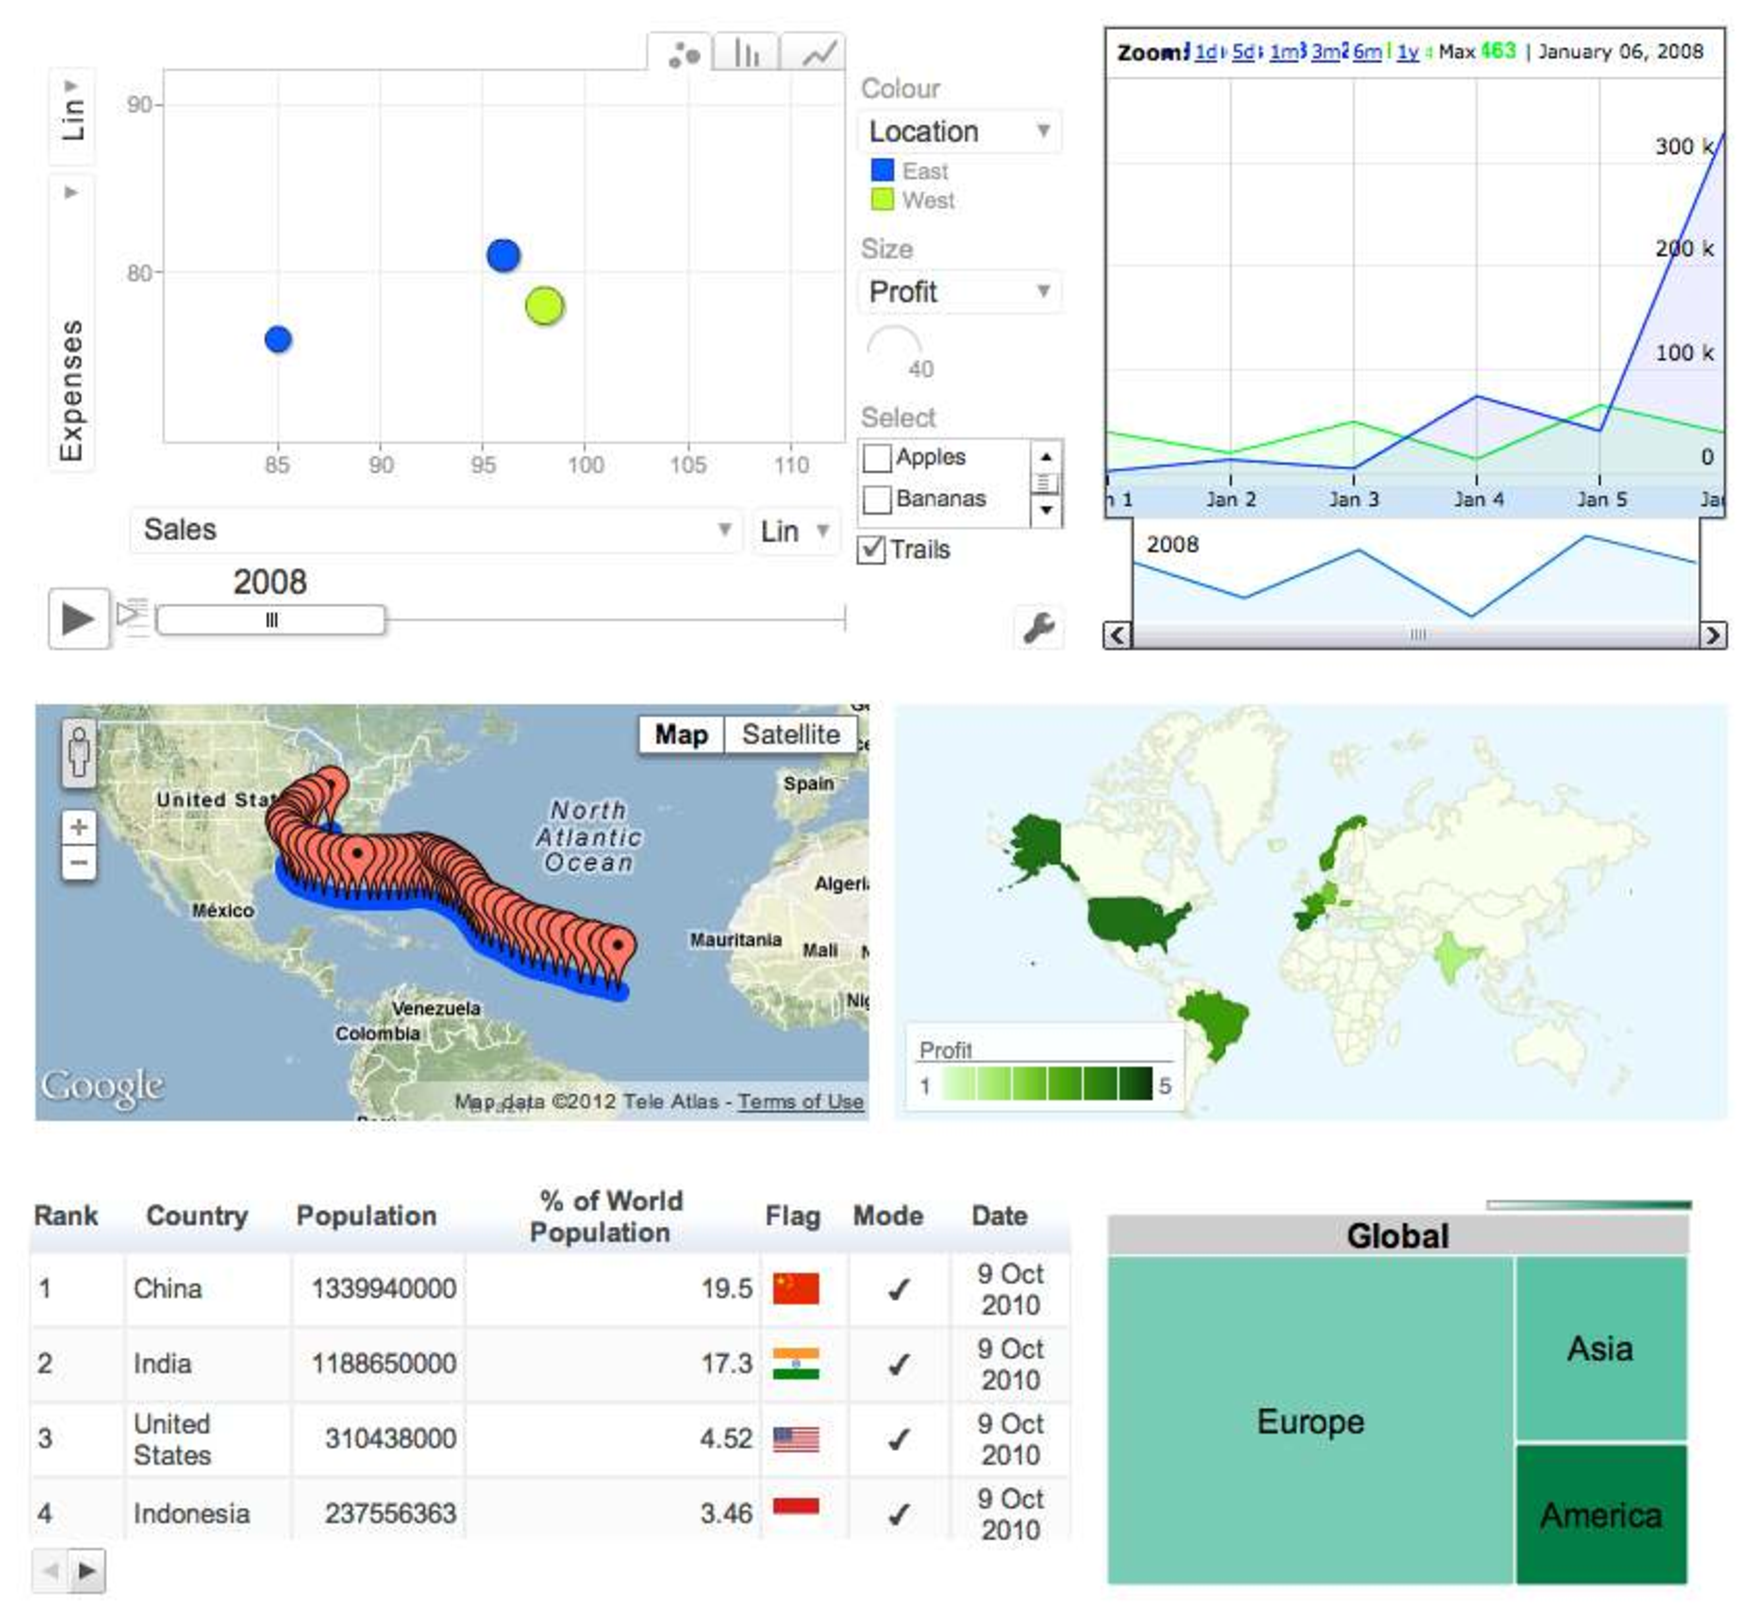
\includegraphics[width=\textwidth]{googleVisDemoPlots.pdf}
\caption{
  Screenshot of the output of \texttt{demo(googleVis)} with 
  \texttt{gvisTreeMap,  gvisTable, gvisMotionChart, gvisGeoMap} from
  top left to bottom right.  
}\label{demos}
\end{center}
\end{figure}


\subsection{Installation}
The \googleVis  package depends on the \rjsonio and
\rsp packages, so we need to install those as well. 
%% Currently the \rjsonio
%% package is not available from CRAN, hence we have to install
%% it from source via: 
%%
%%\begin{verbatim}
%%R> install.packages('RJSONIO', repos='http://www.omegahat.org/R', 
 %%                   type='source')
%%\end{verbatim}
%%Please check the R documentation~\cite{Rinstall} if you are unfamiliar with installing packages from source.
 %%             
%%Following the installation of \rjsonio
We can install \texttt{R.rsp, RJSONIO} and \googleVis in the usual way from CRAN, e.g.:
\begin{verbatim}
R> install.packages(c('R.rsp', 'RJSONIO', 'googleVis'), 
                    repos='http://cran.r-project.org') 
\end{verbatim}

The installation was successful if the
command \texttt{library(googleVis)} gives you the following message:
<<>>=
library(googleVis)
@ 


\subsection{Using the  \googleVis package}

The individual functions of the \googleVis package are documented in
detail in the help pages. Here we will cover more the principals of
the package.

As an example we will show how to generate a motion chart as in  
Figure~\ref{MotionChartGUI}. It works analog for the other
APIs. Further examples are covered in the demos of the \googleVis
package, see also Figure~\ref{demos}. 

The design of the visualisation functions are fairly generic. The name
of the visualisation function is \texttt{'gvis' + ChartType}, so for
the Motion Chart we have: 
\begin{verbatim}
gvisMotionChart(data, idvar='id', timevar='date', options=list())
\end{verbatim}
Here \texttt{data} is the input \texttt{data.frame} and \texttt{idvar}
and \texttt{timevar} specify the column names of the id variable and
time variable for the plot, while display options are set in an
optional list. The options and data requirements follow those of the
Google Visualisation API and are documented in the help pages, see
\texttt{?gvisMotionChart}.  

The output of a \googleVis charting function is a list of lists
containing information about the chart type, chart id and the html
code in a  sub-list with header, chart, caption and footer.

The idea behind this concept is, that users get on one hand side a
complete web page, but on the other hand can extract specific parts,
such as the chart. This is particular helpful if the package functions
are used in solutions where the user wants to feed the visualisation
output into other sites, or would like to embed them into rsp-pages,
see page~\pageref{rspexample}.  

The output of a \googleVis function will be of class \texttt{'gvis'}
and \texttt{'list'}. Generic print (\texttt{print.gvis})  and plot
(\texttt{plot.gvis}) function exist to ease the handle of such objects. 

To illustrate the concept we shall create a motion chart using the Fruits
sample data set.

\subsection{Motion Chart Example}

Following the documentation of the Google Motion Chart API we need a
data set which has at least four columns; one identifying the
variable we would like to plot, one time variable and at least two
numerical variables. Further numerical and character columns are allowed.

As an example we shall use the \texttt{Fruits} data set:
<<>>=
data(Fruits)
Fruits
@

In this case we will use the columns \texttt{'Fruit'} and
\texttt{'Year'} as id and time variable respectively. 


<<>>=
 M <- gvisMotionChart(Fruits, idvar="Fruit", timevar="Year")
@
The output of \texttt{gvisMotionChart} is a list of list as described above
<<>>=
 str(M)
@ 
The first to item of the list contains information about the chart type
used and an individual chart id generated at run time from the chart
type and date:
<<>>=
M$type
M$chartid
@ 
The html list is than split into header, chart, caption and
footer. This allows the user to either extract only certain parts
of the page, or to create a complete html page. 

The header part of the html page has only basic html tags and includes
two rsp-files to provide a  simple framework.
<<>>=
cat(M$html$header)
@ 
The actual Google Visualisation is stored in the \texttt{chart} item
of the html list. 
<<>>=
cat(M$html$chart)
@

A basic chart caption and html footer are the final items of the html list:
<<>>=
cat(M$html$caption)
cat(M$html$footer)
@ 
To display the page locally just type:
\begin{verbatim}
R> plot(M)
\end{verbatim}
The plot method for \texttt{gvis} object will automatically create a
rsp-file in the \texttt{myAnalysis} folder of the \googleVis package
using the type and chart id information of the object and display it
with the local web server of the \rsp package.

Further examples are part of the \googleVis demo. One
example shows how the output of several visualisations can
be incorporated into a single page.


\subsection{Using \texttt{googl{V}is} with \texttt{rsp}}\label{rspexample}
The \rsp package allows the user to integrate R code into html-code,
which together with the \rsp web server are executed at run time.

As mentioned above the R.rsp packages allows us to dynamically
generate documents into static content using R Server Pages. This
means we can mix html and R code to create content on the fly.   As an
example, we can embed the above motion chart into a rsp-page: 
\begin{verbatim}
<html>
<body>
<%=gvisMotionChart(Fruits, idvar="Fruit", timevar="Year")$html$Chart%>
</body>
</html>
\end{verbatim}
You find a few examples a part of the \googleVis package, which can be displayed
via the following R command:
\begin{verbatim}
browseRsp("http://127.0.0.1:8074/library/googleVis/rsp/")
\end{verbatim}
The actual rsp-file is located within the \googleVis package directory, and again R
allows you to find the file with the following R command: 
\begin{verbatim}
filePath(system.file("rsp", package = "googleVis"), "index.rsp")
\end{verbatim}
Please read also the documentation of the \rsp package.

\clearpage

\bibliographystyle{alpha}
\bibliography{googleVis}
\addcontentsline{toc}{section}{References} 

\end{document}


\message{ !name(googleVis.Rnw.tex) !offset(-353) }
